%%%%%%%%%%%%%%%%%%%%%%%%%%%%%%%%%%%%%%%%%
% Beamer Presentation
% LaTeX Template
%----------------------------------------------------------------------------------------
%	PACKAGES AND THEMES
%----------------------------------------------------------------------------------------

\documentclass[notheorems,compress]{beamer}

\mode<presentation> {
\usetheme{Montpellier}

%\usecolortheme{lily}
%\usecolortheme{whale}
%\usecolortheme{dolphin}
%\usecolortheme{seahorse}

\setbeamercovered{transparent}
\usefonttheme[onlymath]{serif}
\setbeamertemplate{navigation symbols}{}
%\setbeamertemplate{footline}{} % To remove the footer line in all slides uncomment this line
%\setbeamertemplate{footline}[page number]
%\setbeamertemplate{background canvas}[vertical shading][bottom=red!10,top=blue!10]
\setbeamertemplate{blocks}[rounded][shadow=true]

%\setbeamertemplate{footline}{%
%  \hfill%
%  \usebeamercolor[fg]{page number in head/foot}%
%  \usebeamerfont{page number in head/foot}%
%  \insertframenumber \,/\,\inserttotalframenumber
%  \kern1em\vskip2pt%
%}

}
%\addtobeamertemplate{headline}{	% title & chaptername (first headline)
%\begin{beamercolorbox}{section in head/foot}
%   \vskip2pt \hspace{2mm} \inserttitle \vskip2pt
%\end{beamercolorbox}
%\begin{beamercolorbox}[colsep=1.5pt,ht=.25ex]{upper separation line head}                   % separator
%\end{beamercolorbox}
%}

\setbeamertemplate{headline}{	% navigation bar of section (second headline)
\begin{beamercolorbox}{section in head/foot}
   \vskip2pt\insertnavigation{\paperwidth}\vskip2pt
\end{beamercolorbox}
\begin{beamercolorbox}[colsep=1.5pt,ht=.3ex]{upper separation line head}  % separator [colsep=1.5pt,ht=.3ex]
\end{beamercolorbox}
}
%\setbeamercolor{upper separation line head}{bg=red}%{shadow theme}

%\defbeamertemplate*{footline}{shadow theme}
%{%
%  \leavevmode%
%  \hbox{\begin{beamercolorbox}[wd=.5\paperwidth,ht=2.5ex,dp=1.125ex,leftskip=.3cm plus1fil,rightskip=.3cm]{author in head/foot}%
%    \usebeamerfont{author in head/foot}\insertshortauthor
%  \end{beamercolorbox}%
%  \begin{beamercolorbox}[wd=.5\paperwidth,ht=2.5ex,dp=1.125ex,leftskip=.3cm,rightskip=.3cm plus1fil]{title in head/foot}%
%    \usebeamerfont{title in head/foot}\insertshorttitle \hfill \insertframenumber\,/\,\inserttotalframenumber%
%  \end{beamercolorbox}}%
%  \vskip0pt%
%}


\setbeamertemplate{footline}
{
  \leavevmode%
  \hbox{%
  \begin{beamercolorbox}[wd=.333333\paperwidth,ht=2.25ex,dp=1ex,center]{author in head/foot}%
    \usebeamerfont{author in head/foot}\insertshortauthor
  \end{beamercolorbox}%
  \begin{beamercolorbox}[wd=.333333\paperwidth,ht=2.25ex,dp=1ex,center]{title in head/foot}%
    \usebeamerfont{title in head/foot}\insertshorttitle \hfill
  \end{beamercolorbox}%
  \begin{beamercolorbox}[wd=.333333\paperwidth,ht=2.25ex,dp=1ex,right]{date in head/foot}%
    \usebeamerfont{date in head/foot}\insertshortdate{}\hspace*{2em}
    \insertframenumber\,/\,\inserttotalframenumber\hspace*{2ex}
  \end{beamercolorbox}}%
  \vskip0pt%
}


\setbeamertemplate{caption}[numbered]
\numberwithin{figure}{section}
\numberwithin{table}{section}
\numberwithin{equation}{section}


\usepackage{amsmath}
\usepackage{graphicx} % Allows including images
\usepackage{booktabs} % Allows the use of \toprule, \midrule and \bottomrule in tables

\usepackage[english]{babel}  % Show english numerate
\usepackage{epsfig,amssymb,amsmath,version}
\usepackage{amssymb,version,graphicx,fancybox,mathrsfs,multirow}
\usepackage{epstopdf}
\usepackage{url,hyperref}

\usepackage{color,xcolor}
\usepackage{cases}
\usepackage{mathtools}
%\usepackage[UTF8,noindent]{ctex}

\setbeamertemplate{theorems}[numbered]
\newtheorem{theorem}{Theorem}
\numberwithin{theorem}{section}
\newtheorem{definition}{Definition}
\numberwithin{definition}{section}
\newtheorem{lemma}{Lemma}
\numberwithin{lemma}{section}
\theoremstyle{example}
\newtheorem{example}{Example}
%\numberwithin{example}{section}


\setbeamertemplate{caption}[numbered]
\numberwithin{figure}{section}
\numberwithin{table}{section}
\numberwithin{equation}{section}


\AtBeginSection[]
{ \begin{frame}
    \frametitle{Overview}
    \tableofcontents[currentsection,hideallsubsections]
  \end{frame}
  \addtocounter{framenumber}{-1}  %目录页不计算页码
}

%\AtBeginSubsection[]
%{
%	\begin{frame}[shrink]
%   \frametitle{Overview}
%	%\thispagestyle{empty}
%	\addtocounter{framenumber}{-1}
%	\tableofcontents[
%	sectionstyle=show/shaded,
%	subsectionstyle=show/shaded/hide]
%\end{frame}
%}

%----------------------------------------------------------------------------------------
%	TITLE PAGE
%----------------------------------------------------------------------------------------

\title[Short title]{Full Title of the Talk} % The short title appears at the bottom of every slide, the full title is only on the title page

\author{John Smith} % Your name
\institute[NU] % Your institution as it will appear on the bottom of every slide, may be shorthand to save space
{
Name of University \\ % Your institution for the title page
\medskip
\textit{name@email.com} % Your email address
}
\date[2020.6.23]{Jun 23, 2020} % Date, can be changed to a custom date


\graphicspath{{./Figures/}}

\begin{document}

%\thispagestyle{empty}
%{\setbeamertemplate{headline}{}
\begin{frame}
\titlepage % Print the title page as the first slide
\end{frame}
%}

\begin{frame}
\frametitle{Overview} % Table of contents slide, comment this block out to remove it
\tableofcontents[hideallsubsections] % Throughout your presentation, if you choose to use \section{} and \subsection{} commands, these will automatically be printed on this slide as an overview of your presentation
\end{frame}

%----------------------------------------------------------------------------------------
%	PRESENTATION SLIDES
%----------------------------------------------------------------------------------------

%------------------------------------------------
\section{First Section} % Sections can be created in order to organize your presentation into discrete blocks, all sections and subsections are automatically printed in the table of contents as an overview of the talk
%------------------------------------------------

\subsection{Subsection Example} % A subsection can be created just before a set of slides with a common theme to further break down your presentation into chunks

\begin{frame}
\frametitle{Paragraphs of Text}
This is paragraphs of text. The quick brown fox jumps over the lazy dog. The quick brown fox jumps over the lazy dog. The quick brown fox jumps over the lazy dog. The quick brown fox jumps over the lazy dog. The quick brown fox jumps over the lazy dog. \\~\\

The quick brown fox jumps over the lazy dog. The quick brown fox jumps over the lazy dog. The quick brown fox jumps over the lazy dog. The quick brown fox jumps over the lazy dog. The quick brown fox jumps over the lazy dog. The quick brown fox jumps over the lazy dog. The quick brown fox jumps over the lazy dog. The quick brown fox jumps over the lazy dog.
\end{frame}

%------------------------------------------------

\begin{frame}
\frametitle{Lists}

\begin{enumerate}
  \item This is a enumerate environment.
  \item This is a enumerate environment.
  \item This is a enumerate environment.
\end{enumerate}

\vspace{2ex}
\begin{itemize}[<+-| alert@+>]
\item This is a itemize environment.
\item This is a itemize environment.
\item This is a itemize environment.
\end{itemize}
\end{frame}

%------------------------------------------------

\begin{frame}
\frametitle{Blocks of Highlighted Text}
\begin{block}{Block Title}
This is the block environment. The quick brown fox jumps over the lazy dog. The quick brown fox jumps over the lazy dog. The quick brown fox jumps over the lazy dog.
\end{block}

\begin{exampleblock}{Block Title}
This is the exampleblock environment. The quick brown fox jumps over the lazy dog. The quick brown fox jumps over the lazy dog.
\end{exampleblock}

\begin{alertblock}{Block Title}
This is the alertblock environment. The quick brown fox jumps over the lazy dog. The quick brown fox jumps over the lazy dog.
\end{alertblock}
\end{frame}

%------------------------------------------------

\begin{frame}
\frametitle{Multiple Columns}
\begin{columns}[c] % The "c" option specifies centered vertical alignment while the "t" option is used for top vertical alignment

\column{0.5\textwidth}
This is a text in first column.
$$E=mc^2$$
\begin{itemize}
\item First item
\item Second item
\end{itemize}

\column{0.5\textwidth}
This text will be in the second column
and on a second tought this is a nice looking
layout in some cases.

\end{columns}
\end{frame}

%------------------------------------------------
\section{Second Section}
%------------------------------------------------

\begin{frame}
\frametitle{Table and Lemma}
\begin{table}
\caption{Table caption}
\begin{tabular}{l l l}
\toprule
Treatments & Response 1 & Response 2 \\
\midrule
Treatment 1 & 0.0003262 & 0.562 \\
Treatment 2 & 0.0015681 & 0.910 \\
Treatment 3 & 0.0009271 & 0.296 \\
\bottomrule
\end{tabular}
\end{table}

\begin{lemma}
This is a lemma environment.
\end{lemma}
\end{frame}


%------------------------------------------------


\begin{frame}[fragile] % Need to use the fragile option when verbatim is used in the slide
\frametitle{Verbatim}
\begin{example}[Theorem Slide Code]
\begin{verbatim}
\begin{frame}
\frametitle{Theorem}
\begin{theorem}[Mass--energy equivalence]
$E = mc^2$
\end{theorem}
\end{frame}\end{verbatim}
\end{example}

\begin{theorem}[Mass--energy equivalence]
$E = mc^2$
\end{theorem}
\end{frame}

%------------------------------------------------

\begin{frame}
\frametitle{Figure}

Uncomment the code on this slide to include your own image from the same directory as the template .TeX file.
\begin{figure}[htp!]
\centering
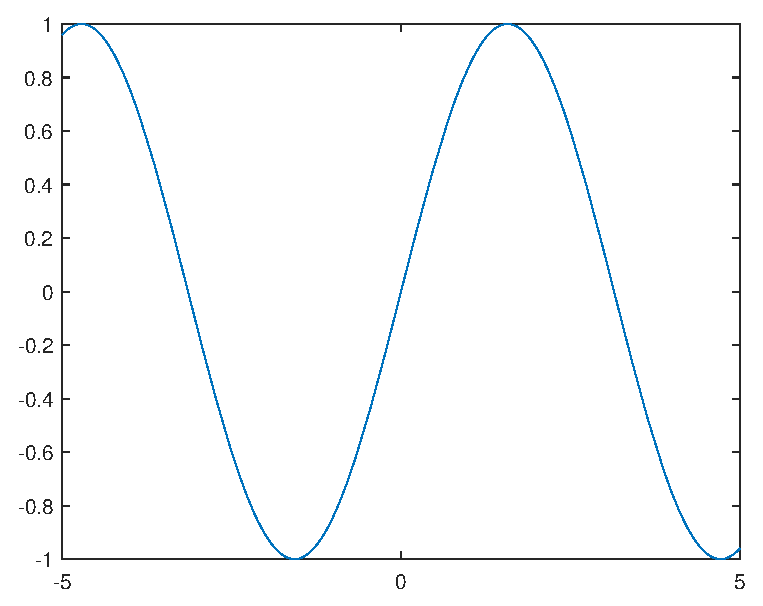
\includegraphics[width=0.6\linewidth]{Image.eps}
\end{figure}
\end{frame}

%------------------------------------------------

\begin{frame}[fragile] % Need to use the fragile option when verbatim is used in the slide
\frametitle{Citation}
An example of the \verb|\cite| command to cite within the presentation:\\~

This statement requires citation \cite{Smith2012}.
\end{frame}

%------------------------------------------------

\begin{frame}
\frametitle{References}
\footnotesize{
\begin{thebibliography}{99} % Beamer does not support BibTeX so references must be inserted manually as below
\bibitem[Smith, 2012]{Smith2012} John Smith. Title of the publication. \emph{Journal Name}, 12(3):45--678, 2012.
\end{thebibliography}
}
\end{frame}



%------------------------------------------------
%\thispagestyle{empty}
%\setbeamertemplate{background canvas}[vertical shading][bottom=white,top=structure.fg!25]
\setbeamertemplate{headline}{}
\begin{frame}
\Huge{\centerline{The End}}
\end{frame}

%----------------------------------------------------------------------------------------

%\thispagestyle{empty}
%\setbeamertemplate{background canvas}[vertical shading][bottom=white,top=structure.fg!25]
%\setbeamertemplate{footline}{}
%\begin{frame}
%\begin{center}
%\Huge \emph{\textcolor[RGB]{128,0,255}{Thanks for your attention!}}
%\end{center}
%\end{frame}


\end{document}

